\documentclass{beamer}

\usepackage[utf8]{inputenc}
\usepackage{fancybox}
\usepackage{environ}

\beamertemplatenavigationsymbolsempty

\title{1.2 Initial-Value Problems}

\subtitle{a lesson for MATH F302 Differential Equations}

\author{Ed Bueler, Dept.~of Mathematics and Statistics, UAF}

\date{\tiny \today}


\usetheme{Pittsburgh}


\begin{document}

\setbeamertemplate{itemize item}{$\bullet$}
\setbeamertemplate{itemize subitem}{$\circ$}


\begin{frame}
\titlepage

\centerline{\tiny for textbook: \, D. Zill, \emph{A First Course in Differential Equations with Modeling Applications}, 11th ed.}
%\color{green!40!blue}
\end{frame}


\begin{frame}{main purpose}

\begin{itemize}
\item the main purpose of differential equations (DEs) in science and engineering is \emph{prediction}
    \begin{itemize}
    \item \emph{models} which are capable of prediction
    \item more on this in section 1.3
    \end{itemize}
\item two things are needed to make a prediction:
\begin{align*}
\begin{matrix}
\text{precise description} \\
\text{of rate of change}
\end{matrix} && \iff && &\text{differential equation} \\
\begin{matrix}
\text{knowledge} \\
\text{of current state}
\end{matrix} && \iff && &\text{initial conditions}
\end{align*}
\end{itemize}
\end{frame}


\begin{frame}{prediction models}

\begin{itemize}
\item DEs do \emph{not} ``know the future'' as perfect predictions
\item they are \emph{models} which are \emph{capable} of prediction
\item next two slides are examples
\item \emph{do not worry about understanding the specific equations on the next two slides}
\end{itemize}
\end{frame}


\begin{frame}{amazing-accuracy prediction model}

\begin{columns}
\begin{column}{0.55\textwidth}
\begin{itemize}
\item Newton's theory of gravitation gives remarkably-accurate predictions of planets, satellites, and space probes
\item the DEs at right for many particles interacting by gravity
\item coupled, nonlinear, 2nd-order ODEs for the position $\mathbf{r}_i$ of each object with mass $m_i$
\item adding corrections for relativity makes these predictions practically perfect
\end{itemize}
\end{column}
\begin{column}{0.45\textwidth}
$$\frac{d^2 \mathbf{r}_i}{dt^2} = G \sum_{j\ne i} \frac{m_i m_j}{|\mathbf{r}_j - \mathbf{r}_i|^3} (\mathbf{r}_j - \mathbf{r}_i)$$

\medskip

\quad \tiny \href{https://en.wikipedia.org/wiki/Equations_of_motion}{\texttt{en.wikipedia.org/wiki/Equations\_of\_motion}}
\end{column}
\end{columns}
\end{frame}


\begin{frame}{pretty-good prediction model}

\begin{columns}
\begin{column}{0.5\textwidth}
\begin{itemize}
\item \emph{weather prediction} uses a system of PDEs for fluids
\item predictions have been refined over time by comparing prediction to what actually happened
\item now we have $\sim$6 days of good predictions
\item equations at right
\item more on models in section 1.3; we will start with single ODEs not systems of PDEs!
\end{itemize}
\end{column}
\begin{column}{0.5\textwidth}
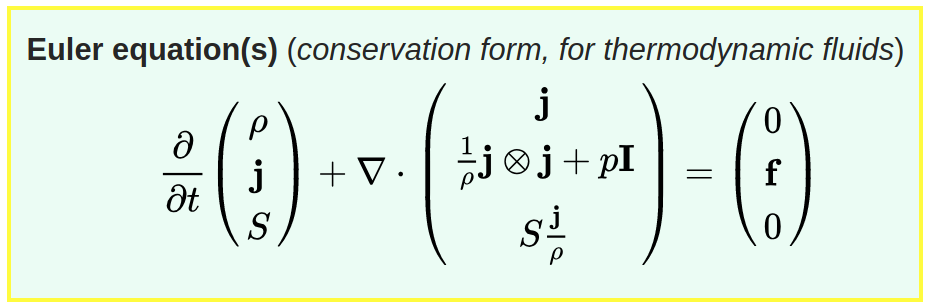
\includegraphics[width=\textwidth]{figs/euler-equations}

\medskip

\quad \tiny \href{https://en.wikipedia.org/wiki/Euler_equations_(fluid_dynamics)}{\texttt{en.wikipedia.org/wiki/}}

\qquad \href{https://en.wikipedia.org/wiki/Euler_equations_(fluid_dynamics)}{\texttt{Euler\_equations\_(fluid\_dynamics)}}
\end{column}
\end{columns}
\end{frame}


\begin{frame}{example 1}

\begin{itemize}
\item section 1.2 is about initial conditions and how they ``pick out'' one prediction (solution) from all the solutions of a differential equation
\item first order
\end{itemize}
\end{frame}

\begin{frame}{example 2}

\begin{itemize}
\item 2nd order
\end{itemize}
\end{frame}

\begin{frame}{general IVP}

\begin{itemize}
\item the general form of an initial-value problem for an ordinary differential equation (ODE IVP) is equation (1) at the start of section 1.2:
\begin{align*}
\frac{d^n y}{dx^n} &= f(x,y,y',\dots,y^{(n-1)}) \\
y(x_0) &= y_0 \\
y'(x_0) &= y_1 \\
   &\vdots \\
y^{(n-1)}(x_0) &= y_{n-1}
\end{align*}
\end{itemize}
\end{frame}

\begin{frame}{Z}

\begin{itemize}
\item X
\end{itemize}
\end{frame}

\begin{frame}{Z}

\begin{itemize}
\item X
\end{itemize}
\end{frame}



\begin{frame}{expectations}

\textbf{expectations}:  to learn this material, just watching this video is \emph{not} enough
\begin{itemize}
\item you need to \emph{read} section 1.2 in the textbook
\item you need to \emph{do} the WebAssign exercises for section 1.2
\item you need to \emph{look around} for other videos and related content; start with the Week 1 page at \href{https://bueler.github.io/math302/}{bueler.github.io/math302}
\end{itemize}
\end{frame}


\end{document}

